\begin{fact}
	Nous avons les cas initiaux suivants.
	
	\begin{itemize}[label = \small\textbullet]
		\item Il n'y a aucun rebond si et seulement si $\sigma_S \in \intervalC{- \dfrac{\pi}{2} - \theta}{- \dfrac{\pi}{2}}$.
		
		\item La bille va directement vers $F$ si et seulement si $\sigma_S = \dfrac{\pi}{2} - \theta + \tau$.

		\item Le 1\ier{} rebond se fait sur $\setgeo*{d}{1}$ si et seulement si $\sigma_S \in \intervalOC{\dfrac{\pi}{2} - \theta + \tau}{\pi} \cup \intervalO{- \pi}{- \dfrac{\pi}{2} - \theta}$.

		\item Le 1\ier{} rebond se fait sur $\setgeo*{d}{2}$ si et seulement si $\sigma_S \in \intervalO{- \dfrac{\pi}{2}}{\dfrac{\pi}{2} - \theta + \tau}$.
	\end{itemize}

\end{fact}

\begin{proof}
	Tout est contenu dans les deux dessins suivants où $\setgeo*{D}{k} \, /\!/ \, \setgeo*{d}{k}$ pour $k \in \{ 1 \,; 2\}$.

	\medskip

	\begin{center}
		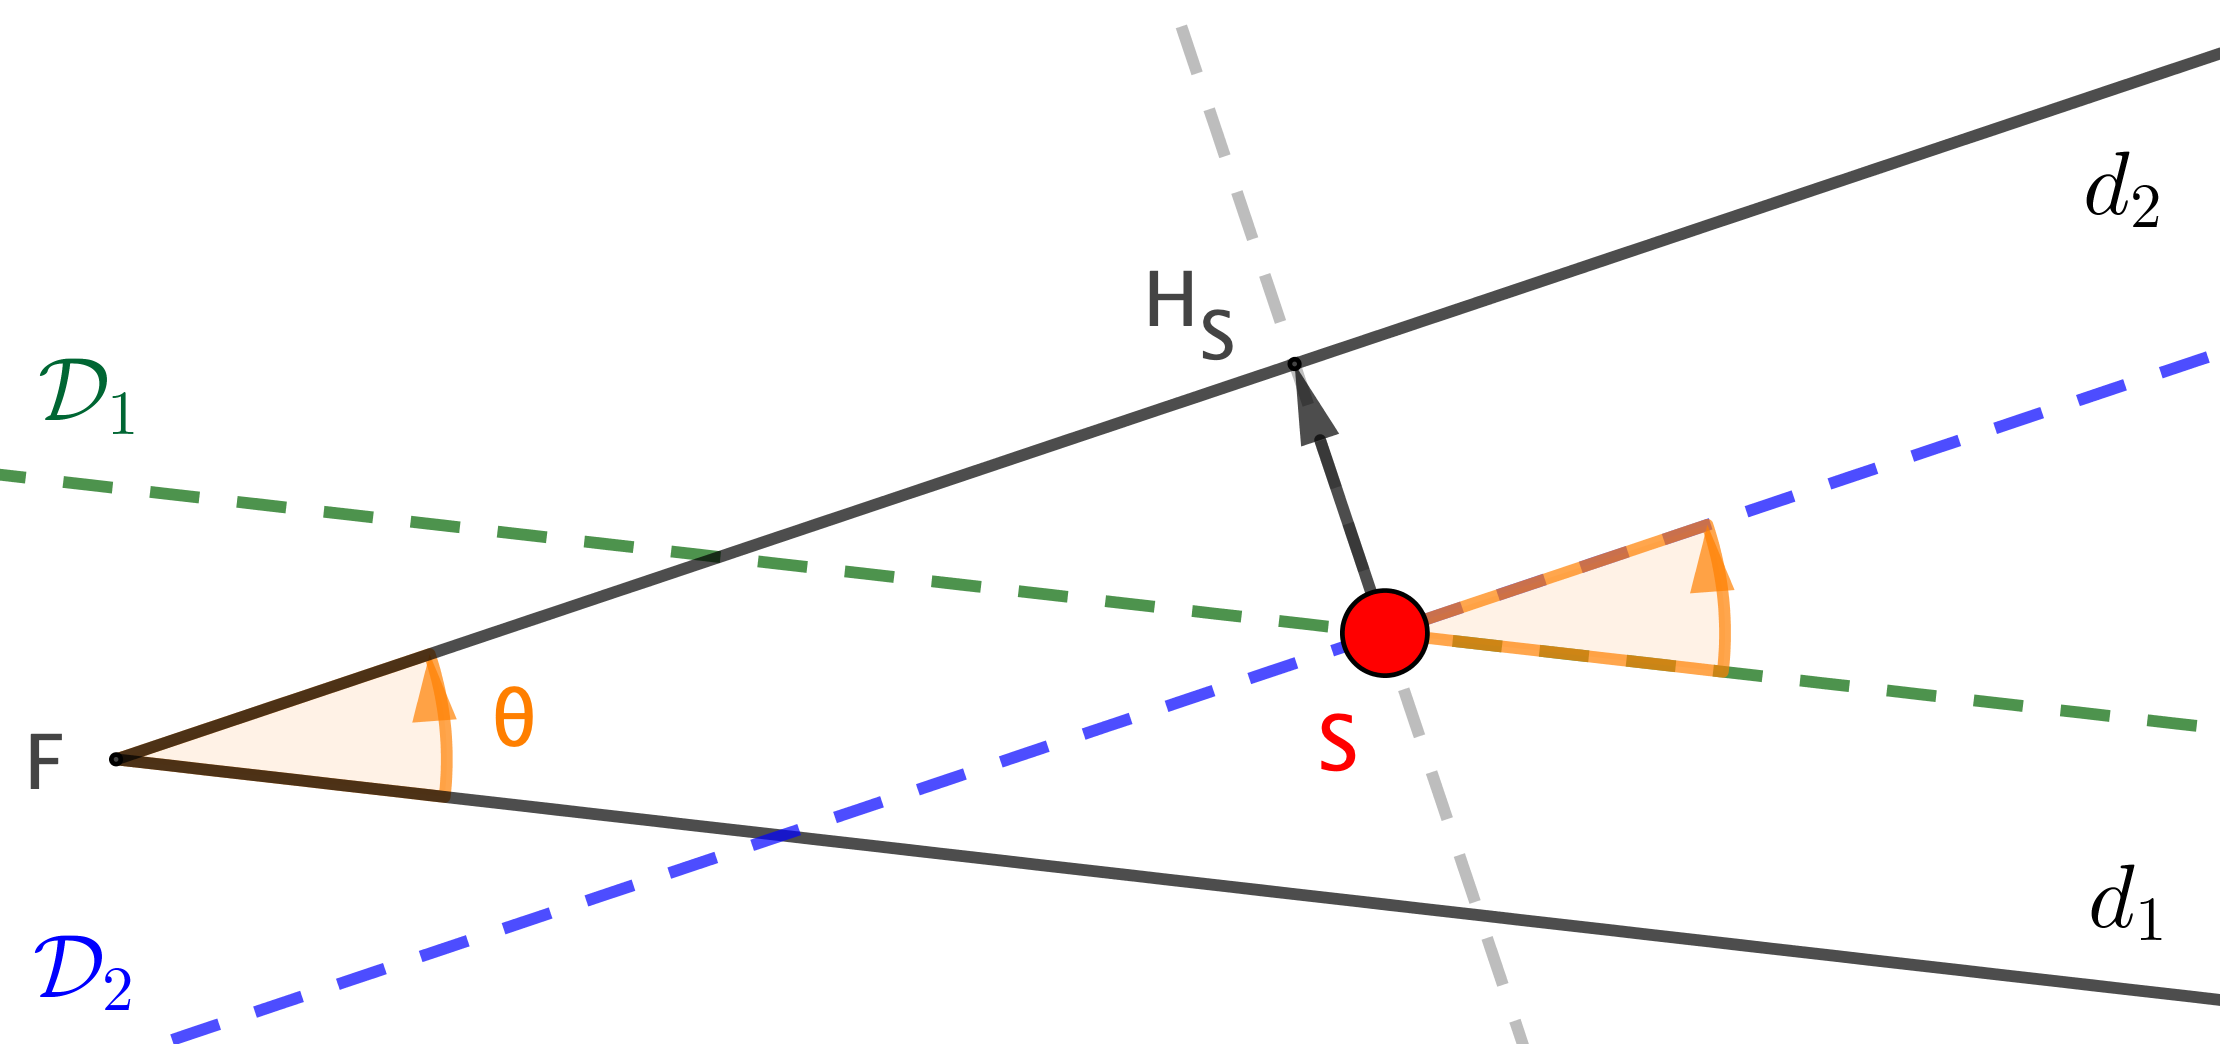
\includegraphics[width=12cm]{content/proof-no-bounce.png}

		\itshape\small
		Aucun 1\ier{} rebond
	\end{center}

	\medskip

	\begin{center}
		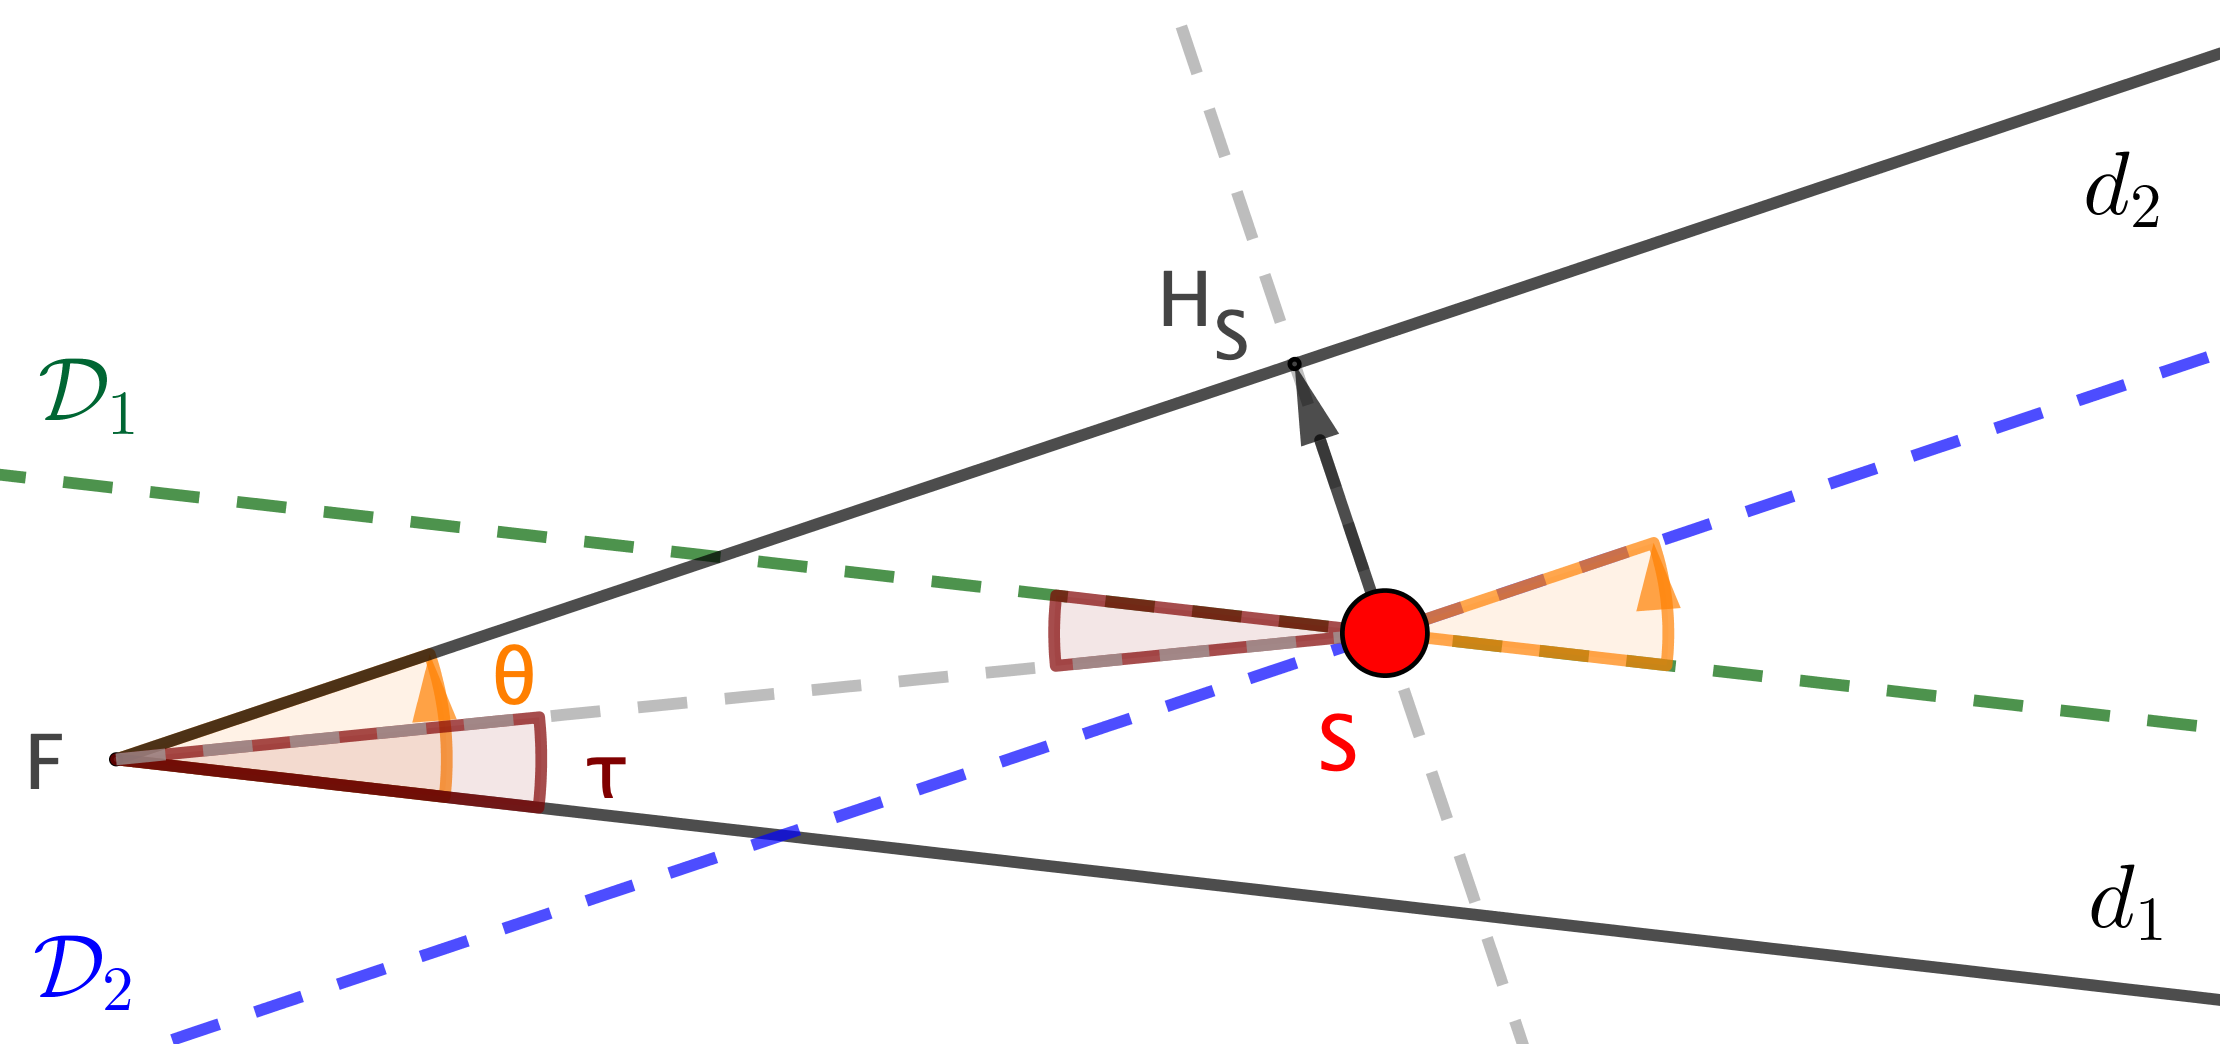
\includegraphics[width=12cm]{content/proof-1st-bounce-somewhere.png}

		\itshape\small
		Les autres cas
	\end{center}
\end{proof}


Il nous reste juste à traiter les cas d'un 1\ier{} rebond se faisant sur $\setgeo*{d}{1}$ et $\setgeo*{d}{2}$ respectivement.

\begin{tcolorbox}
	\centering\itshape
	
	En fait, nous n'avons besoin de traiter que la situation d'un 1\ier{} rebond sur $\setgeo*{d}{2}$.
\end{tcolorbox}

En effet, une fois ceci étudié, l'autre cas s'obtiendra avec le même type de raisonnement excepté que l'on projettera $S$ sur $\setgeo*{d}{1}$ au lieu de $\setgeo*{d}{2}$.
